\documentclass[aspectratio=169]{beamer}
\usepackage[utf8]{inputenc}
\usepackage[T1]{fontenc}
\usepackage{booktabs}
\usepackage{colortbl}
\usepackage{graphicx}
\usepackage{xcolor}
\usepackage{tikz}
\usetikzlibrary{positioning,arrows.meta,shapes.geometric}
\usepackage{pgfplots}
\pgfplotsset{compat=1.18}
\usepackage{amsmath}
\usepackage{tcolorbox}
\tcbuselibrary{skins}

\definecolor{cdark}{HTML}{0D2137}
\definecolor{cmid}{HTML}{065A82}
\definecolor{cteal}{HTML}{02C39A}
\definecolor{clight}{HTML}{E8F4F8}
\definecolor{ctext}{HTML}{1A2E40}
\definecolor{cmuted}{HTML}{607D8B}
\definecolor{cwarn}{HTML}{F4A261}
\definecolor{cgap}{HTML}{E63946}
\definecolor{caccent}{HTML}{A0BFD0}
\definecolor{cbg2}{HTML}{028090}

\usetheme{default}
\usecolortheme{default}
\setbeamertemplate{navigation symbols}{}
\usefonttheme{professionalfonts}
\setbeamerfont{frametitle}{size=\large,series=\bfseries}
\setbeamercolor{frametitle}{fg=cdark,bg=white}
\setbeamercolor{normal text}{fg=ctext}
\setbeamercolor{background canvas}{bg=white}
\setbeamercolor{item}{fg=cteal}

\addtobeamertemplate{frametitle}{}{%
  \vspace{-4pt}\textcolor{cteal}{\hrule height 1.5pt}\vspace{3pt}}

\setbeamertemplate{footline}{%
  \leavevmode\hbox{%
    \begin{beamercolorbox}[wd=0.85\paperwidth,ht=2.2ex,dp=1ex,leftskip=4pt]{normal text}%
      \tiny\color{cmuted}An Pham \textbar{} LIRMM--ADVANSE \textbar{} Luc \& Reda%
    \end{beamercolorbox}%
    \begin{beamercolorbox}[wd=0.15\paperwidth,ht=2.2ex,dp=1ex,right,rightskip=6pt]{normal text}%
      \scriptsize\color{cmuted}\insertframenumber/\inserttotalframenumber%
    \end{beamercolorbox}}}

\setbeamertemplate{itemize item}{\color{cteal}\textbullet}
\setbeamertemplate{itemize subitem}{\color{cmid}--}
\setlength{\leftmargini}{1em}

\tikzset{
  flowbox/.style={rounded corners, draw=cmid, fill=clight, align=center,
    minimum height=0.9cm, text width=2.8cm, font=\footnotesize},
  flowarrow/.style={-Latex, thick, color=cmid}
}

\title{\textbf{Mixed-Length Shapelets to KMeans}}
\subtitle{Picoclimate Example from Raw Data}
\author{An Pham}
\institute{LIRMM--ADVANSE, Universit\'e de Montpellier}
\date{May 27, 2026}

\begin{document}

% --- Slide 1 ---
{\setbeamercolor{background canvas}{bg=cdark}
\begin{frame}[plain]
\begin{tikzpicture}[remember picture,overlay]
  \fill[cteal](current page.north west)rectangle([xshift=6pt]current page.south west);
\end{tikzpicture}
\vspace{1.1cm}
{\color{white}\huge\bfseries Mixed-Length Shapelets to KMeans}\\[5pt]
{\color{cteal}\large\itshape Picoclimate Example from Raw Data}\\[8pt]
{\color{caccent}\small Explainable Clustering for Spatio-Temporal Data}\\[0.6cm]
{\color{cmid}\rule{5.6cm}{0.8pt}}\\[5pt]
{\color{caccent}\footnotesize\textbf{An Pham}\quad|\quad LIRMM--ADVANSE\quad|\quad Supervisors: Luc \& Reda}\\[2pt]
{\color{caccent}\footnotesize May 27, 2026}
\end{frame}}

% --- Slide 2 ---
\begin{frame}{Raw Measurements to Window Features}
\begin{center}
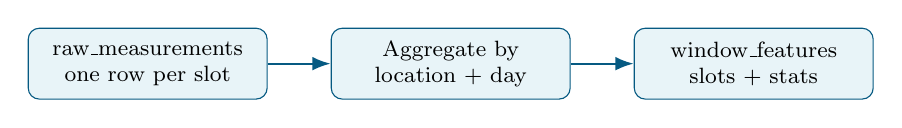
\begin{tikzpicture}[node distance=1.0cm and 0.8cm]
  \node[flowbox] (raw) {raw\_measurements\\one row per slot};
  \node[flowbox, right=of raw] (agg) {Aggregate by\\location + day};
  \node[flowbox, right=of agg] (win) {window\_features\\slots + stats};

  \draw[flowarrow] (raw) -- (agg);
  \draw[flowarrow] (agg) -- (win);
\end{tikzpicture}
\end{center}
\vspace{4pt}
{\scriptsize\itshape Slot rows are aggregated into one daily window per location.}
\end{frame}

% --- Slide 3 ---
\begin{frame}{Example Row: raw\_measurements.csv (Truncated)}
\scriptsize
\begin{tabular}{@{}lllllll@{}}
\toprule
\textbf{timestamp} & \textbf{location} & \textbf{slot} & \textbf{air\_temp} & \textbf{humidity} & \textbf{wind} & \textbf{pressure} \\
\midrule
2025-09-01 06:00 & loc\_000 & morning & 50.0 & 5.0 & 17.226 & 969.0 \\
\bottomrule
\end{tabular}
\vspace{6pt}
\begin{itemize}\footnotesize\setlength\itemsep{4pt}
  \item Each row is one location + one time slot (morning/noon/afternoon/night).
  \item These rows become a 4-slot daily window in \texttt{window\_features.csv}.
\end{itemize}
\end{frame}

% --- Slide 4 ---
\begin{frame}{Example Row: window\_features.csv (Truncated)}
\scriptsize
\resizebox{\textwidth}{!}{%
\begin{tabular}{@{}llllllll@{}}
\toprule
\textbf{location} & \textbf{date} & \textbf{present} & \textbf{air\_temp\_s1} & \textbf{wind\_s1} & \textbf{air\_temp\_s2} & \textbf{wind\_s2} & \textbf{true\_regime} \\
\midrule
loc\_049 & 2025-09-24 & 0.9348 & 50.0 & 12.516 & 50.0 & 12.045 & traffic\_peak \\
\bottomrule
\end{tabular}}
\vspace{6pt}
\begin{itemize}\footnotesize\setlength\itemsep{4pt}
  \item Slot columns (\texttt{\_\_slot\_1..\_\_slot\_4}) are the shapelet input.
  \item Mean/std/trend columns exist but are not used in the shapelet pipeline.
\end{itemize}
\end{frame}

% --- Slide 5 ---
\begin{frame}{Shapelet Input Vector (Picoclimate)}
\begin{columns}[T,onlytextwidth]
  \column{0.6\textwidth}
  \begin{itemize}\footnotesize\setlength\itemsep{4pt}
    \item Build one 1D vector per window using only slot columns.
    \item Example (truncated):
  \end{itemize}
  \vspace{2pt}
  \begin{tcolorbox}[enhanced,boxrule=1pt,arc=2pt,colback=clight,colframe=cmid]
    \scriptsize
    $x =$ [slot1: temp, humidity, wind, ...,
    slot2: temp, humidity, wind, ..., slot4: ...]
  \end{tcolorbox}
  \column{0.4\textwidth}
  \begin{itemize}\footnotesize\setlength\itemsep{4pt}
    \item This is \textbf{not} a single-variable series.
    \item It is a flattened multivariate window.
  \end{itemize}
\end{columns}
\end{frame}

% --- Slide 6 ---
\begin{frame}{Ordering Matters: Variable vs Slot}
\begin{columns}[T,onlytextwidth]
  \column{0.48\textwidth}
  \begin{tcolorbox}[enhanced,boxrule=1pt,arc=2pt,colback=clight,colframe=cwarn]
    \footnotesize\textbf{Bad (variable-grouped)}\\[2pt]
    \scriptsize\ttfamily
    temp\_s1, temp\_s2, temp\_s3, temp\_s4,\\
    humidity\_s1, humidity\_s2, ...
  \end{tcolorbox}
  \column{0.48\textwidth}
  \begin{tcolorbox}[enhanced,boxrule=1pt,arc=2pt,colback=clight,colframe=cmid]
    \footnotesize\textbf{Good (slot-grouped)}\\[2pt]
    \scriptsize\ttfamily
    temp\_s1, humidity\_s1, wind\_s1, ...,\\
    temp\_s2, humidity\_s2, wind\_s2, ...
  \end{tcolorbox}
\end{columns}
\vspace{4pt}
{\scriptsize\itshape Slot-wise ordering keeps local shapelets temporally natural.}
\end{frame}

% --- Slide 7 ---
\begin{frame}{Mixed-Length Shapelets to Distance Features}
\begin{columns}[T,onlytextwidth]
  \column{0.6\textwidth}
  \begin{itemize}\footnotesize\setlength\itemsep{4pt}
    \item Short lengths only (e.g., 2--6) for 4-slot windows.
    \item Semi-exhaustive candidates + pruning (low variance, duplicates, correlation).
    \item Each shapelet yields one feature: minimum distance to the window.
  \end{itemize}
  \column{0.4\textwidth}
  \begin{block}{Distance mapping}
  \vspace{-6pt}
  \[
  \phi_j(x) = \min_{t} \lVert x[t:t+L_j] - s_j \rVert_2
  \]
  \[
  X_{shapelet} \in \mathbb{R}^{N \times m}
  \]
  \end{block}
\end{columns}
\end{frame}

% --- Slide 8 ---
\begin{frame}{Candidate Strategy (Semi-Exhaustive + Pruning)}
\begin{itemize}\footnotesize\setlength\itemsep{4pt}
  \item Generate all candidates for short lengths on a subset of rows.
  \item Drop low-variance and duplicate shapelets.
  \item Keep top candidates by distance-dispersion score.
  \item Prune highly correlated candidates and keep a compact dictionary.
\end{itemize}
\end{frame}

% --- Slide 9 ---
\begin{frame}{Clustering Input and Options}
\begin{center}
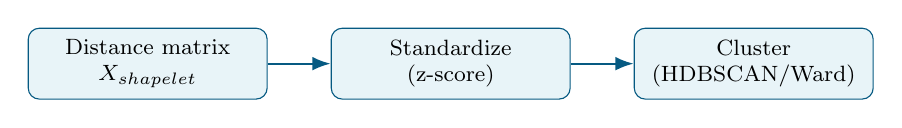
\begin{tikzpicture}[node distance=1.0cm and 0.8cm]
  \node[flowbox] (dist) {Distance matrix\\$X_{shapelet}$};
  \node[flowbox, right=of dist] (scale) {Standardize\\(z-score)};
  \node[flowbox, right=of scale] (k) {Cluster\\(HDBSCAN/Ward)};

  \draw[flowarrow] (dist) -- (scale);
  \draw[flowarrow] (scale) -- (k);
\end{tikzpicture}
\end{center}
\vspace{4pt}
{\scriptsize\itshape KMeans remains a baseline; HDBSCAN and Ward are primary options.}
\end{frame}

% --- Slide 10 ---
\begin{frame}{Picoclimate Summary (May 27, 2026)}
\begin{columns}[T,onlytextwidth]
  \column{0.48\textwidth}
  \begin{itemize}\footnotesize\setlength\itemsep{4pt}
    \item Config: max\_rows=120, eval\_rows=40, max\_pool=1000, target\_shapelets=200
    \item 1,500 windows; 87 slot columns; 188 shapelets
    \item KMeans best k=3 (silhouette 0.0391)
    \item Ward silhouette 0.0292 at k=3
    \item HDBSCAN unavailable in current env (install pending)
  \end{itemize}
  \column{0.52\textwidth}
  \begin{center}
    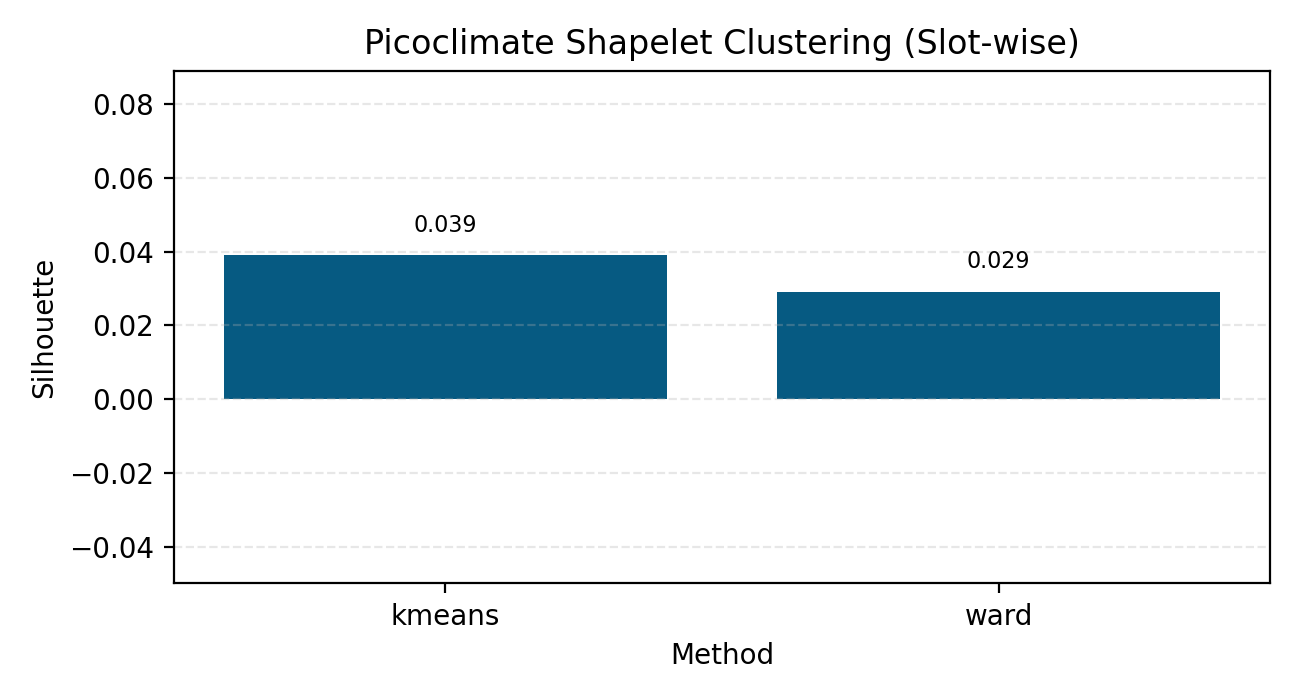
\includegraphics[width=\textwidth]{../../../scripts/figures/picoclimate_shapelet_results_2026-05-27.png}
  \end{center}
\end{columns}
\end{frame}

% --- Slide 11 ---
\begin{frame}{Explanation Stage (Transparent)}
\begin{columns}[T,onlytextwidth]
  \column{0.52\textwidth}
  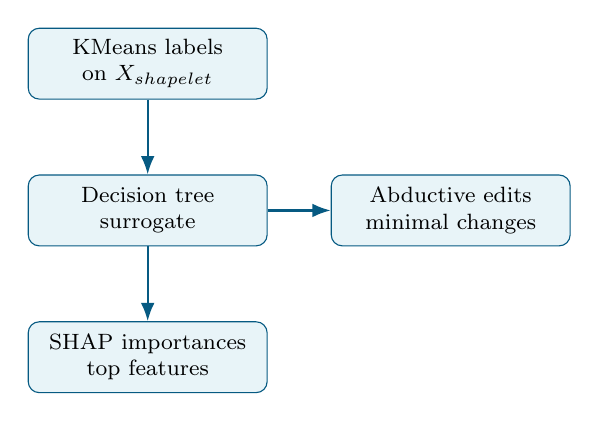
\begin{tikzpicture}[node distance=0.95cm and 0.8cm]
    \node[flowbox] (labels) {KMeans labels\\on $X_{shapelet}$};
    \node[flowbox, below=of labels] (tree) {Decision tree\\surrogate};
    \node[flowbox, below=of tree] (shap) {SHAP importances\\top features};
    \node[flowbox, right=of tree] (abduct) {Abductive edits\\minimal changes};

    \draw[flowarrow] (labels) -- (tree);
    \draw[flowarrow] (tree) -- (shap);
    \draw[flowarrow] (tree) -- (abduct);
  \end{tikzpicture}
  \column{0.48\textwidth}
  \begin{itemize}\footnotesize\setlength\itemsep{4pt}
    \item Surrogate learns cluster rules in shapelet space.
    \item SHAP ranks which shapelet distances drive the label.
    \item Mean/std/trend features are used only for interpretation.
    \item Abductive edits show minimal changes to switch cluster.
  \end{itemize}
\end{columns}
\end{frame}

% --- Slide 12 ---
\begin{frame}{Interpretation for T=4 Slots}
\begin{itemize}\footnotesize\setlength\itemsep{4pt}
  \item Shapelets act as local multivariate motifs, not long temporal patterns.
  \item Slot-wise ordering keeps motifs aligned to neighboring time slots.
  \item Statistics (mean/std/trend) provide global context after clustering.
  \item Single-variable shapelets are viable only with long sequences.
\end{itemize}
\end{frame}

\end{document}
